\section{Programación del PLC}
\label{sec:program.plc}

Para la programación del PLC se usará el software de desarrollo que proporciona la compañía ABB en su web\footnote{http://new.abb.com/plc/automationbuilder/platform/software}. La versión usada en este proyecto del Automation Builder es la última liberada hasta la fecha, la 1.1.0.824, como se indicó en la sección \ref{eleccion_PLC} este software es gratuito para el uso que le vamos a dar.\\
    \begin{figure}[H]
            \centering
            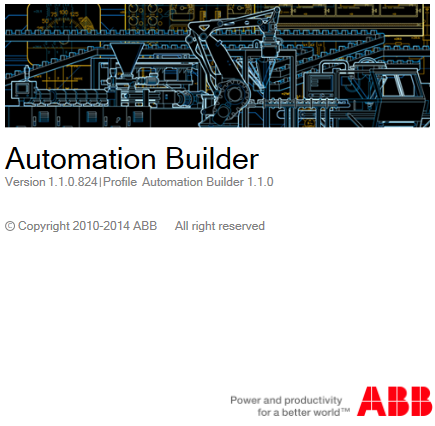
\includegraphics[width=0.4\textwidth]{images/PLC/ABB.png}
            \caption{Splash Screen del Automation Builder}
            \label{fig:PLC_splashabb}
    \end{figure}
Las acciones que debe realizar el PLC son las siguientes:

\begin{itemize}
	\item{Controlar la temperatura del extrusor.}
	\item{Controlar motor del husillo.}
	\item{Leer información del sensor de diámetro.}
	\item{Almacenar la información tomada en un fichero de datos.}
	\item{Visualizar en una página web el estado de la producción.}
\end{itemize}

Para realizar el software que gestione el PLC, se usará una máquina de estados, en la que pasando por diversas fases, se irán ejecutando las acciones de control. Deberemos entrar en modo producción mediante la activación de una variable, con la que si estamos en producción, pasaremos por los distintos estados, mientras no estemos en producción, las salidas digitales y valores de consigna de los PID, estarán reseteados a cero como medida de seguridad. Una vez que entremos en producción, el primer paso será inicializar el programa, generaremos el nombre del fichero donde almacenaremos los datos. Se elije un nombre en el que se usa año, mes, día y minuto para identificar la producción, es decir, tendría un formato \textit{YYMMDDmm.CSV}.\\

El formato elegido para almacenar la información es el de valores separados por coma (CSV). El motivo por el cual se elije este formato es debido a su estandarización y que almacena los datos de forma tabular en texto plano. Gracias a esto, podremos abrir el fichero CSV con cualquier editor de texto y otros programas de hojas de cálculo, para el posterior análisis de los datos, que es uno de los objetivos del proyecto. Por lo tanto, el formato CSV es el idóneo para poder trabajar en el futuro con los datos almacenados.\\

En esta inicialización, también se genera la cabecera del fichero CSV , que es la primera fila del fichero, en donde indicará la información que contiene cada columna. La información almacenada en el fichero CSV será la siguiente:

\begin{itemize}
	\item{\textbf{Time Stamp: }Es una secuencia de caracteres en las que se indican hora y fecha de un evento ocurrido. Se almacena con el  formato YY-MM-DD HH:MM:SS. Con esta información podremos tener una trazabilidad del filamento almacenado y en caso de producirse un error, ver el momento concreto del mismo.}
	\item{\textbf{Temperaturas: }Valores con las temperaturas del dado y el husillo en la zona de alimentación. De esta manera se comprueba que la temperatura no sufre algún cambio drástico durante el proceso, que puede ser causante de un problema en la calidad final del filamento (X e Y).}
	\item{\textbf{Diámetros: }Se almacenan los diámetros medidos por el sensor. En este caso se van a poner dos sensores de diámetro para hacer una medición en los dos ejes del filamento.}
	\item{\textbf{Información varia: }Se puede almacenar cualquier información que nosotros deseemos en un futuro.}
\end{itemize}

Los siguientes pasos dentro de la máquina de estados, será generar el fichero CSV y en caso de que no se produzca ningún error,	 se almacenará la cabecera en el fichero CSV, para pasar a la producción como tal.\\
Se controlará la temperatura del dado, se registrarán los valores de diámetros y temperaturas y se irán almacenando en el fichero CSV. El control del motor del husillo se hará de forma manual desde la visualización online.\\

Una vez que se tiene una idea de cómo va a ser el programa, se desarrolla un diagrama con la máquina de estados.

    \begin{figure}[H]
            \centering
            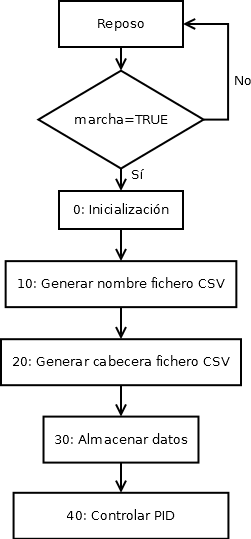
\includegraphics[width=0.25\textwidth]{images/PLC/diagrama.png}
            \caption{Diagrama de estados}
            \label{fig:plc_estados}
    \end{figure}


\subsection{Controlar temperatura extrusor}
\label{sec:plc_PID}

Para controlar la temperatura del extrusor se va a implementar un regulador PID. Los reguladores del tipo PID, añaden tres acciones de regulación,... BLA BLA BLA BLA BLA BLA\cite{PID}\\


Para poder implementar correctamente un regulador PID, será necesario conocer la planta del sistema que queremos regular. En nuestro caso es el sistema de calentamiento del dado, por ello, deberemos modelar primeramente el sistema con el que estamos trabajando.
    \begin{figure}[H]
            \centering
            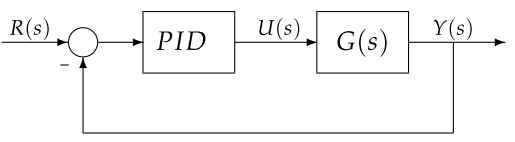
\includegraphics[width=0.4\textwidth]{images/PLC/sistema.png}
            \caption{Sistema con un regulador PID}
            \label{fig:plc_sistema}
    \end{figure}

Con ayuda del programa que estamos desarrollando en el PLC haremos las siguientes tareas:

\begin{itemize}
	\item{Registrar temperaturas del dado.}
	\item{Encender de forma controlada la resistencia de calentamiento.}
	\item{Analizar los datos obtenidos.}
\end{itemize}

Tenemos que ver como se comporta el sistema en lazo abierto, sin ningún tipo de control. Partiendo de una temperatura ambiente, se irán registrando los valores de las temperaturas para a continuación encender la resistencia de calentamiento y ver cómo la temperatura va aumentando a medida que pasa el tiempo. Una vez que la temperatura sobrepase un valor que nosotros establezcamos, pararemos el experimento.\\

Con ayuda del lenguaje de programación Python y varias herramientas de análisis de datos como son: ipython,scipy, pandas y numpy, analizaremos los datos obtenidos. Las gráficas peresentadas a continuación, así como los cálculos están realizadas con esta herramienta.

    \begin{figure}[H]
            \centering
            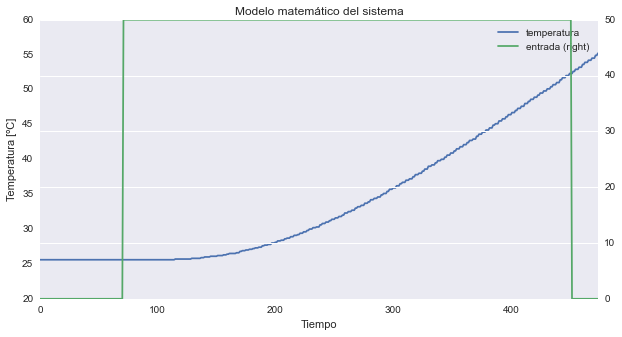
\includegraphics[width=0.75\textwidth]{images/PLC/modelado/modelado_9_1.png}
            \caption{Respuesta del sistema en lazo abierto}
            \label{fig:plc_lazo_abierto}
    \end{figure}

Calcularemos cual es la ecuación que mejore se ajuste a nuestros datos y tendremos el polinomio que caracteriza nuestro sistema.
    \begin{figure}[H]
            \centering
            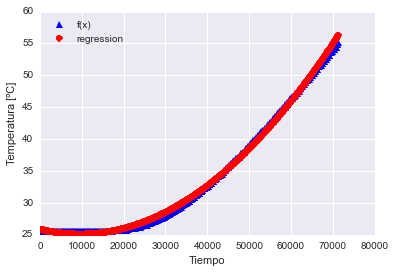
\includegraphics[width=0.5\textwidth]{images/PLC/modelado/modelado_13_1.png}
            \caption{Ajuste de la recta}
            \label{fig:plc_lazo_abierto2}
    \end{figure}
$$P_x=  25.9459 -1.5733 \cdot 10^{-4} \cdot X - 8.18174 \cdot 10^{-9} \cdot X^2$$

Si calculamos la transformada de laplace del sistema, obtenemos la planta de nuestro sistema, con la cual podremos implementar el regulador PID:
$$G_s = \frac{25.95 \cdot S^2 - 0.00015733 \cdot S + 1.63635 \cdot 10^{-8}}{S^3}$$

Aplicando el método de sintonizacion de Ziegler-Nichols basado en la curva reacción calcularemos el PID para poder regular correctamente el sistema.Este método consiste en estudiar el sistema en lazo abierto con escalón unitario, calculamos parámetros como la máxima pendiente de la curva y el retardo, y establecemos con ellos las ganancias del controlador PID\cite{PID}.Nos da de manera rápida unos valores de $K_p$, $K_i$ y $K_d$ orientativos, para que podamos ajustar correctamente el controlador. Con ayuda de la herramienta Open Source Octave, calcularemos los valores de ganancia que serán los que apliquemos a nuestro regulador.

\Cpp
\begin{lstlisting}
pkg load control
%los datos en la funcion tf() debe ser el numerador y denominador de nuestro sistema.
H=tf([25.95 0.000157333 1.63635E-8],[1 0 0 0]);
step(H);
dt=0.150;
t=0:dt:65;
y=step(H,t);
dy=diff(y)/dt;
[m,p]=max(dy);
yi=y(p);
ti=t(p);
L=ti-yi/m
Tao=(y(end)-yi)/m+ti-L
Kp=1.2*Tao/L
Ti=2*L;
Td=0.5*L;
Ki=Kp/ti;
Kd=Kp*Td;
\end{lstlisting}

En esta primera iteración, los datos obtenidos son los siguientes:
$K_p = 6082.6$ $K_i=93.868 K_d=38.9262$

Con lo que nuestro regulador tiene la siguiente ecuación característica:

$$G_s = \frac{38.9262 \cdot S^2 + 6082.6 \cdot S + 93.868}{S}$$

Una vez que tenemos las ganancias de nuestro regulador PID, volvemos a realizar el experimento de calentar la resistencia hasta un valor de temperatura deseado, en este caso 80ºC y vemos cual es la respuesta de nuestro sistema:

    \begin{figure}[H]
            \centering
            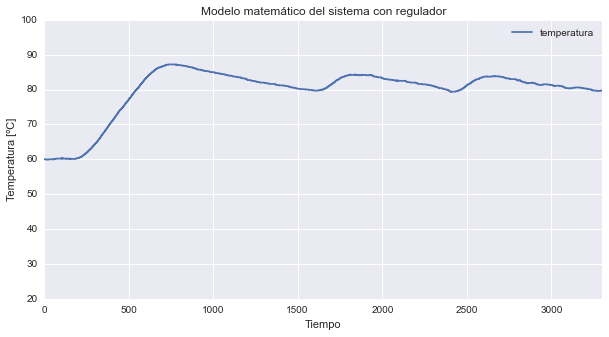
\includegraphics[width=0.75\textwidth]{images/PLC/modelado/modelado_26_1.png}
            \caption{Respuesta del sistema con PID. Iteracción 1}
            \label{fig:plc_PID1}
    \end{figure}

Como podemos objservar en la imagen \ref{fig:plc_PID1} tenemos una sobreoscilación sobre el setpoint elevada:

$$M_{p}=\frac{T_{max}-Setpoint}{Setpoint} \cdot 100 = \frac{87.20-80}{80} \cdot 100 = 9\%$$ 

Siendo el error en régimen  permanente de 3.70.\\
Una vez introducido el controlador, la temperatura tiende a estabilizarse, sin embargo tiene mucha sobreoscilación. Por ello aumentaremos los valores de $K_i$ y $K_d$, siendo los valores de esta segunda iteracción los siguientes:
$K_p = 6082.6$ $K_i=103.25 K_d=51.425$


Realizando una segunda iteracción en el cálculo de nuestro regulador obtenemos lo siguiente:

    \begin{figure}[H]
            \centering
            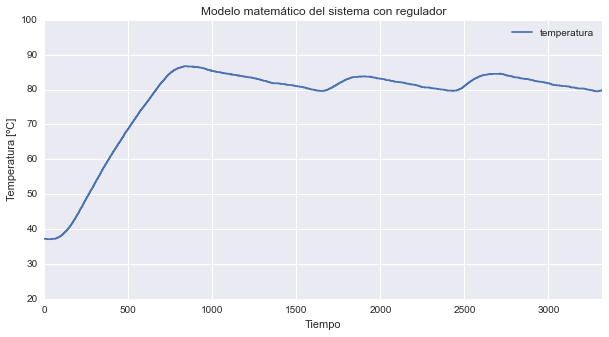
\includegraphics[width=0.75\textwidth]{images/PLC/modelado/modelado_30_1.png}
            \caption{Respuesta del sistema con PID. Iteracción 2}
            \label{fig:plc_PID2}
    \end{figure}
Esta vez los resultados son algo mejores:
$$M_{p}=\frac{T_{max}-Setpoint}{Setpoint} \cdot 100 = \frac{86.70-80}{80} \cdot 100 = 8.38\%$$ 
Siendo el error en régimen permanente de 3.50.\\
En esta segunda iteracción hemos logrado bajar la sobreoscilación inicial, pero tenemos mayor error en regimen permanente. Por ello volvemos a aumentar los valores de $K_i$ y $K_d$ siendo los valores de esta tercera iteracción los siguientes:
$K_p = 6082.6$ $K_i=121.64 K_d=60$

Realizando una tercera iteracción en el cálculo de nuestro regulador obtenemos lo siguiente:

    \begin{figure}[H]
            \centering
            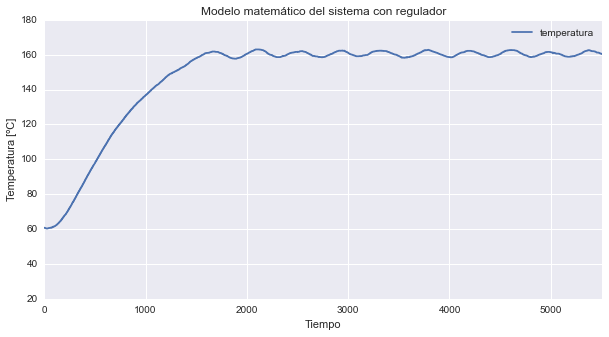
\includegraphics[width=0.75\textwidth]{images/PLC/modelado/modelado_34_1.png}
            \caption{Respuesta del sistema con PID. Iteracción 3}
            \label{fig:plc_PID3}
    \end{figure}
Esta vez los resultados son algo mejores:
$$M_{p}=\frac{T_{max}-Setpoint}{Setpoint} \cdot 100 = \frac{163-160}{160} \cdot 100 = 1.88\%$$ 
Siendo el error en régimen permanente de 1.30\\
En este caso, se puso un setpoint de 160ºC. Como vemos, la sobreoscilación inicial ha disminuido en comparación con la anterior iteracción y el error en regimen permanente es menor. Para intentar minimar el error, aumentaremos únicamente el valor de $K_i$. Siendo los valores de esta cuarta iteracción del regulador los siguientes:
    $K_p = 6082.6$ $K_i=121.64 K_d=150$

Realizando una cuarta iteracción en el cálculo de nuestro regulador obtenemos lo siguiente:

    \begin{figure}[H]
            \centering
            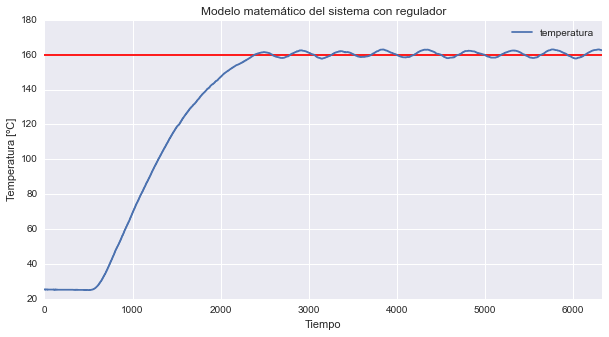
\includegraphics[width=0.75\textwidth]{images/PLC/modelado/modelado_38_1.png}
            \caption{Respuesta del sistema con PID. Iteracción 4}
            \label{fig:plc_PID4}
    \end{figure}
Esta vez los resultados son algo mejores:
$$M_{p}=\frac{T_{max}-Setpoint}{Setpoint} \cdot 100 = \frac{163-160}{160} \cdot 100 = 1.88\%$$ 
Siendo el error en régimen permanente de 1.10\\

Por lo tanto, el regulador que cumple con las especificaciones deseadas tiene la siguiente ecuación característica:
$$G_s = \frac{150 \cdot S^2 + 6082.6 \cdot S + 121.64}{S}$$

\subsection{Leer información del sensor de diámetro}
\label{sec:plc_diametro}

Los sensores de diámetro están conectados a dos entradas analógicas de tensión del PLC. Será necesario unir la señal de masa (GND) del PLC con la del sensor, para que la referencia al nivel de tensión 0v sea la misma, posteriormente, la salida del sensor de diámetro, se conectará con la entrada analógica del PLC.\\

El PLC convierte el valor de tensión comprendido entre un rango de 0-10V a un valor numérico, a través de un conversor analógico a digital (ADC) de 10bits, es decir, tenemos una resolución de:

$$ Resolucion=\frac{ V_{max} } {2^{10} } = \frac{10}{1024} = 9.76 mV$$

Si acudimos a la ayuda que nos ofrece el programa de ABB, podemos observar los valores que asigna el ADC:

\begin{table}[H]
\centering
\begin{tabular}{|c|c|c|}
\hline
{\bf Intervalo}                   & {\bf 0 ... 10V}                                                   & \multicolumn{1}{l|}{{\bf Valor digital}}                       \\ \hline
Desbordamiento                    & \textgreater 11.7589                                              & 32767                                                         \\ \hline
Valor de medición desmasiado alto & \begin{tabular}[c]{@{}c@{}}11.7589\\ .\\ .\\ 10.0004\end{tabular} & \begin{tabular}[c]{@{}c@{}}32511\\ .\\ .\\ 27649\end{tabular} \\ \hline
Intervalo normal                  & \begin{tabular}[c]{@{}c@{}}10.000\\ .\\ .\\ 0.0004\end{tabular}   & \begin{tabular}[c]{@{}c@{}}27648\\ .\\ .\\ 1\end{tabular}     \\ \hline
\end{tabular}
\caption{Valores de conversión del ADC}
\label{tab:reso_adc}
\end{table}

En nuestro caso, vamos a trabajar en el rango de intervalo normal, para poder saber el diámetro que nos está dando el sensor, deberemos leer la entrada analógica y convertir el valor décimal a un valor de tensión, es decir, convertir el valor digital a analogico, (DAC), para ello, cogemos los valores del intervalo normal de la tabla \ref{tab:reso_adc} y calcular la ecuación de la recta que lo caracteriza.

    \begin{figure}[H]
            \centering
            \includegraphics[width=0.75\textwidth]{images/PLC/dac.png}
            \caption{Ecuación: $Y=3.6168 \cdot 10^{-4} \cdot X$}
            \label{fig:plc_DAC}
    \end{figure}

Con este valor, y el calculado en \pageref{fig:sens_regre} somos capaces de leer el valor del diámetro, para ello, prograremos un bloque que llamaremos linealizacion, en la que tendrá los siguientes parámetros:

\begin{itemize}
    \item{\textbf{Entradas:}}
        \begin{itemize}
            \item{\textbf{IN:}Entrada analógica donde se encuentra físicamente el sensor}
            \item{\textbf{AD:}Valor del DAC calculado anteriormente}
            \item{\textbf{M y B:} Valores de la ecuación de la recta, que minimizan el error medido por el sensor}         
        \end{itemize}
    \item{\textbf{Salida:}}
        \begin{itemize}
            \item{\textbf{OUT:} Valor real de la magnitud medida por el sensor.}
        \end{itemize}
\end{itemize}